\documentclass[11pt,a4paper,]{article}
\usepackage{lmodern}
\usepackage{amssymb,amsmath}
\usepackage{ifxetex,ifluatex}
\usepackage{fixltx2e} % provides \textsubscript
\ifnum 0\ifxetex 1\fi\ifluatex 1\fi=0 % if pdftex
  \usepackage[T1]{fontenc}
  \usepackage[utf8]{inputenc}
\else % if luatex or xelatex
  \ifxetex
    \usepackage{mathspec}
  \else
    \usepackage{fontspec}
  \fi
  \defaultfontfeatures{Ligatures=TeX,Scale=MatchLowercase}
\fi
% use upquote if available, for straight quotes in verbatim environments
\IfFileExists{upquote.sty}{\usepackage{upquote}}{}
% use microtype if available
\IfFileExists{microtype.sty}{%
\usepackage{microtype}
\UseMicrotypeSet[protrusion]{basicmath} % disable protrusion for tt fonts
}{}
\usepackage[margin=1in]{geometry}
\usepackage{hyperref}
\hypersetup{unicode=true,
            pdftitle={Who we are affects how we vote},
            pdfauthor={Rob J Hyndman and Di Cook},
            pdfborder={0 0 0},
            breaklinks=true}
\urlstyle{same}  % don't use monospace font for urls
\usepackage[style=authoryear-comp]{biblatex}

\addbibresource{references.bib}
\usepackage{longtable,booktabs}
\usepackage{graphicx,grffile}
\makeatletter
\def\maxwidth{\ifdim\Gin@nat@width>\linewidth\linewidth\else\Gin@nat@width\fi}
\def\maxheight{\ifdim\Gin@nat@height>\textheight\textheight\else\Gin@nat@height\fi}
\makeatother
% Scale images if necessary, so that they will not overflow the page
% margins by default, and it is still possible to overwrite the defaults
% using explicit options in \includegraphics[width, height, ...]{}
\setkeys{Gin}{width=\maxwidth,height=\maxheight,keepaspectratio}
\IfFileExists{parskip.sty}{%
\usepackage{parskip}
}{% else
\setlength{\parindent}{0pt}
\setlength{\parskip}{6pt plus 2pt minus 1pt}
}
\setlength{\emergencystretch}{3em}  % prevent overfull lines
\providecommand{\tightlist}{%
  \setlength{\itemsep}{0pt}\setlength{\parskip}{0pt}}
\setcounter{secnumdepth}{5}
% Redefines (sub)paragraphs to behave more like sections
\ifx\paragraph\undefined\else
\let\oldparagraph\paragraph
\renewcommand{\paragraph}[1]{\oldparagraph{#1}\mbox{}}
\fi
\ifx\subparagraph\undefined\else
\let\oldsubparagraph\subparagraph
\renewcommand{\subparagraph}[1]{\oldsubparagraph{#1}\mbox{}}
\fi

%%% Use protect on footnotes to avoid problems with footnotes in titles
\let\rmarkdownfootnote\footnote%
\def\footnote{\protect\rmarkdownfootnote}

%%% Change title format to be more compact
\usepackage{titling}

% Create subtitle command for use in maketitle
\providecommand{\subtitle}[1]{
  \posttitle{
    \begin{center}\large#1\end{center}
    }
}

\setlength{\droptitle}{-2em}

  \title{Who we are affects how we vote}
    \pretitle{\vspace{\droptitle}\centering\huge}
  \posttitle{\par}
    \author{Rob J Hyndman and Di Cook}
    \preauthor{\centering\large\emph}
  \postauthor{\par}
    \date{}
    \predate{}\postdate{}
  
%% Any special functions or other packages can be loaded here.

\usepackage[no-weekday]{eukdate}
\usepackage{sourceserifpro}
\usepackage[scaled=0.86]{DejaVuSansMono}
\usepackage{float,bm,setspace}
\setstretch{1.2}

%% CAPTIONS
\RequirePackage{caption}
\DeclareCaptionStyle{italic}[justification=centering]
 {labelfont={bf},textfont={it},labelsep=colon}
\captionsetup[figure]{style=italic,format=hang,singlelinecheck=true}
\captionsetup[table]{style=italic,format=hang,singlelinecheck=true}

%% GRAPHICS
\RequirePackage{graphicx}
\setcounter{topnumber}{2}
\setcounter{bottomnumber}{2}
\setcounter{totalnumber}{4}
\renewcommand{\topfraction}{0.85}
\renewcommand{\bottomfraction}{0.85}
\renewcommand{\textfraction}{0.15}
\renewcommand{\floatpagefraction}{0.8}

%% BIBLIOGRAPHY

\makeatletter
\@ifpackageloaded{biblatex}{}{\usepackage[style=authoryear-comp, backend=biber, natbib=true]{biblatex}}
\makeatother
\ExecuteBibliographyOptions{bibencoding=utf8,minnames=1,maxnames=3, maxbibnames=99,dashed=false,terseinits=true,giveninits=true,uniquename=false,uniquelist=false,doi=false, isbn=false,url=true,sortcites=false}

\DeclareFieldFormat{url}{\texttt{\url{#1}}}
\DeclareFieldFormat[article]{pages}{#1}
\DeclareFieldFormat[inproceedings]{pages}{\lowercase{pp.}#1}
\DeclareFieldFormat[incollection]{pages}{\lowercase{pp.}#1}
\DeclareFieldFormat[article]{volume}{\mkbibbold{#1}}
\DeclareFieldFormat[article]{number}{\mkbibparens{#1}}
\DeclareFieldFormat[article]{title}{\MakeCapital{#1}}
\DeclareFieldFormat[inproceedings]{title}{#1}
\DeclareFieldFormat{shorthandwidth}{#1}
% No dot before number of articles
\usepackage{xpatch}
\xpatchbibmacro{volume+number+eid}{\setunit*{\adddot}}{}{}{}
% Remove In: for an article.
\renewbibmacro{in:}{%
  \ifentrytype{article}{}{%
  \printtext{\bibstring{in}\intitlepunct}}}

\makeatletter
\DeclareDelimFormat[cbx@textcite]{nameyeardelim}{\addspace}
\makeatother
\renewcommand*{\finalnamedelim}{%
  %\ifnumgreater{\value{liststop}}{2}{\finalandcomma}{}% there really should be no funny Oxford comma business here
  \addspace\&\space}

\begin{document}
\maketitle

\hypertarget{intro}{%
\section{Introduction}\label{intro}}

We often hear commentary about voting patterns --- people in their 20s without kids are more likely to be left wing, migrants are more conservative, wealthier people tend to favour the conservative parties, and so on. These might be built on myth and stereotypes. There is open data available from each election and from regular national censuses; this data can be used to examine just what are the indicators for voting tendency.

Voting tendencies can change over time. For example, if wealth was a good predictor of conservative voting in the 2001 election, is it still a good predictor in 2019? Australia has changed in many ways over the last two decades. Rising house prices, country-wide improvements in education, an ageing population, and a decline in religious affiliation, are just some of the ways we have changed. At the same time, political power has moved back and forth between the two major parties. How much can we attribute changes in political power to changes in who we are?

\hypertarget{census-and-electoral-data}{%
\section{Census and electoral data}\label{census-and-electoral-data}}

The Census provides data on electoral socio-demographics, and vote counts in each electorate can be obtained from Australian federal elections. However, joining these two data sources is difficult because the Censuses are not held at the same time as the elections. Between 2001 and 2016 there were six elections and four Censuses, as shown in the timeline below.

\begin{figure}[H]

{\centering 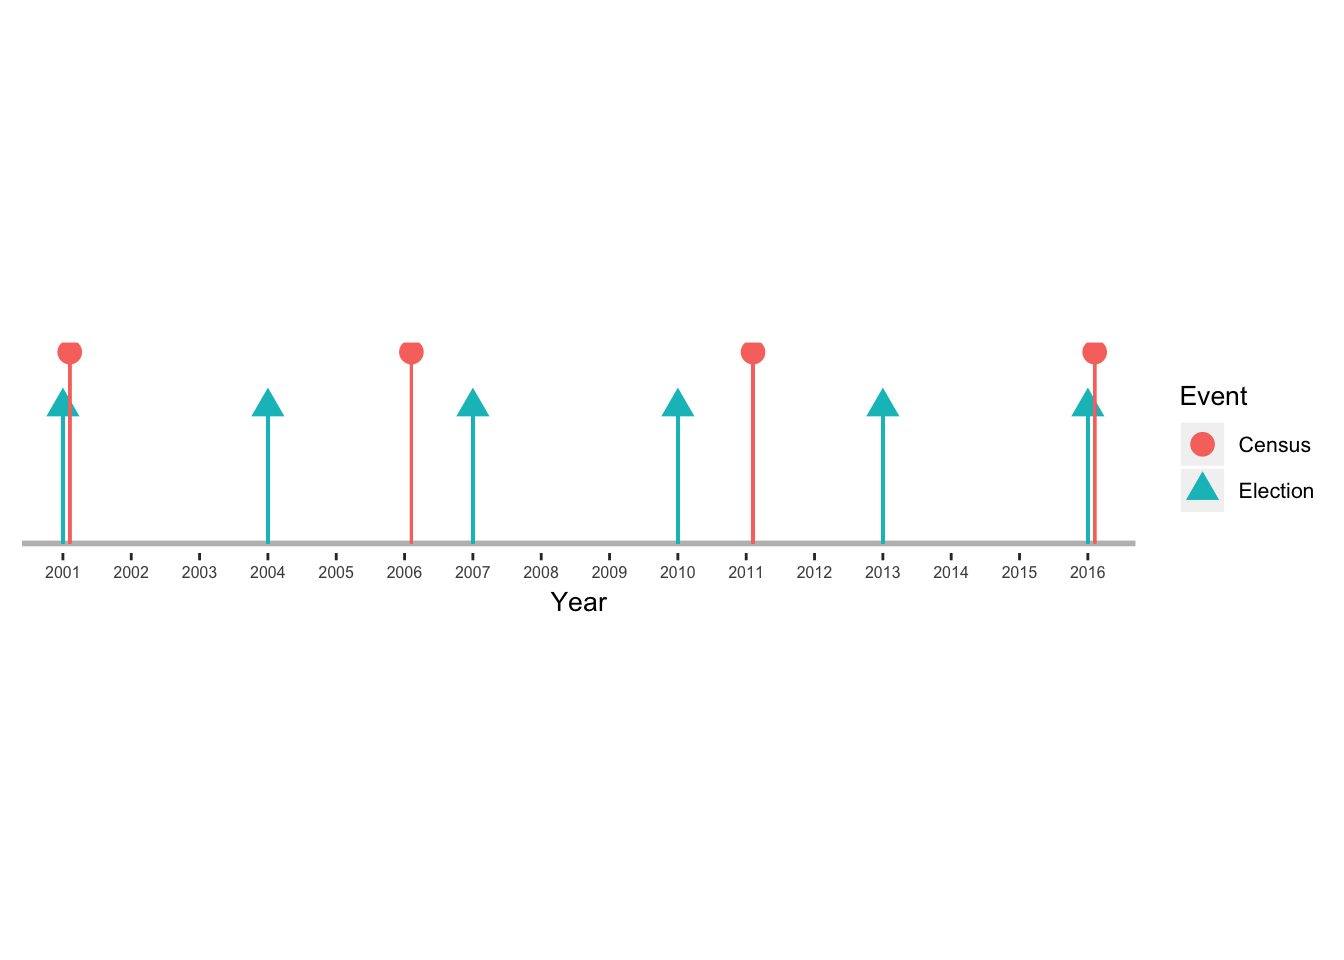
\includegraphics[width=0.9\linewidth]{elections_conversation_files/figure-latex/timeline-1} 

}

\caption{Timeline of Australian elections and Censuses. They do not always occur in the same year.}\label{fig:timeline}
\end{figure}

Not only can an electorate change between the last Census and an election, but even the electorate boundaries can change. Some electorates can disappear altogether and new electorates can arise. Electoral boundaries are redistributed regularly by the AEC, meaning that only in the years where both a Census and an election occur are all boundaries likely to match --- the case for the 2001 and 2016 elections. So we first had to estimate what the socio-demographic characteristics of an electorate would have been at the time of each election using a complicated method of interpolation over time and geography. This method uses Census information from both before and after the election of interest, and information from neighbouring electorates when boundaries have changed.

\hypertarget{modelling}{%
\section{2PP Modelling}\label{modelling}}

A simple way to measure voting patterns is to consider the two-party preferred (2PP) vote, which is based on the tally of preferences for the Labor and Liberal candidates, ignoring all other candidates. By convention, this is recorded as a percentage preference in favour of the Liberal party --- for example, a 2PP value of 45\% indicates that 45\% of voters ranked the Liberal candidate higher than the Labor candidate, while the remaining 55\% ranked them in the reverse order.

We consider how various socio-demographic variables obtained from Census data can be used to explain the 2PP values for each of the 150 electorates in each of the federal elections between 2001 and 2016.

Many of the socio-demographic variables have changing scales over the years. For example, inflation-adjusted median rental prices increased across almost all electorates, with median rent of 200 dollars per week placing an electorate in the 90th percentile in 2001, but only the 30th percentile in 2016. In order for socio-demographic effects to be comparable across years, all socio-demographic variables were standardized.

There are dozens of socio-demographic variables available in the Censuses, with many variables representing similar information about an electorate. So we combined some variables to avoid redundant information. For example, our ``Incomes'' variable is a combination of median personal income, household income and family income.

We are using data at the electorate level. The results do not directly address the voting intentions of individuals.

Each election was modelled separately, to allow us to see any changes over time, and to account for changing electorate boundaries. In this article, we highlight the variables with the strongest relationship to the two-party preferred vote, or which have had substantial changes over time. The full analysis is available at \url{https://robjhyndman.com/publications/elections/}.

\hypertarget{country-wide-trend}{%
\subsection*{Country-wide trend}\label{country-wide-trend}}
\addcontentsline{toc}{subsection}{Country-wide trend}

\begin{figure}[H]

{\centering 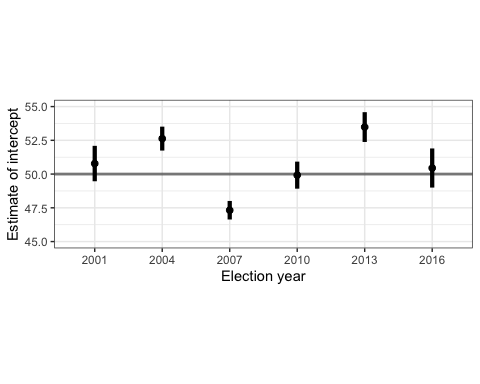
\includegraphics{elections_conversation_files/figure-latex/plotintercept-1} 

}

\caption{Estimated intercept for each election, which represents the two-party preferred vote for an electorate with average characteristics.}\label{fig:plotintercept}
\end{figure}

First, we show the estimated two-party preferred vote for an ``average'' electorate. Figure \ref{fig:plotintercept} shows that the baseline of party preference has varied over the elections, with the biggest swing occurring in the 2007 election where the mean electorate shifted more than five percentage points in favour of the Labor party. The dots represent the estimated 2PP value, and the lines indicate a 95\% confidence interval providing a guide to the uncertainty in the estimate.

\hypertarget{age}{%
\subsection*{Age}\label{age}}
\addcontentsline{toc}{subsection}{Age}

\begin{figure}[H]

{\centering \includegraphics{elections_conversation_files/figure-latex/age-1} 

}

\caption{Estimated age effect for each election, which represents the impact of electorate median age on the two-party preferred vote. Higher values indicate a }\label{fig:age}
\end{figure}

Regions comprising more older people are often believed to be more conservative, and indeed we found that electorates with a higher median age are more likely to support the Liberal party --- although this effect is significant only in 2007 and 2010.

Figure \ref{fig:age} shows the effect of median age on the 2PP vote. The vertical scale can be interpreted as a score measuring how much the 2PP vote differs between an average electorate, and an electorate with median age in the top third of all electorates.

\begin{itemize}
\tightlist
\item
  Would it be possible to show how the correlation changes for different age brackets (ie. younger voters = more Labor, and this swings more to Liberal as the age brackets gets older)?
\item
  If not, can you go into more detail specific age brackets? Eg. Is it the over-65s that skew Liberal?
\end{itemize}

\hypertarget{income-and-unemployment}{%
\subsection*{Income and unemployment}\label{income-and-unemployment}}
\addcontentsline{toc}{subsection}{Income and unemployment}

\begin{figure}[H]

{\centering \includegraphics{elections_conversation_files/figure-latex/income-1} 

}

\caption{Estimated age effect for each election, which represents the impact of electorate median age on the two-party preferred vote. Higher values indicate a }\label{fig:income}
\end{figure}

Typically the Labor party campaigns on more progressive policies, which often include tax reform that adversely affects higher income earners, and more generous social assistance programs. Perhaps it is due to these policies that higher income electorates appear more likely to support the Liberal party, as the \texttt{Incomes} factor has a positive effect on Liberal preference (see row 1 in Figure \ref{fig:partresplot1}). This effect is significant in every election aside from 2004, where it is only marginally insignificant (\(p = 0.0613\)). Unemployment however, is not as influential. In 2001 and 2004, electorates with higher unemployment align with Labor, but over time this shifts towards support for the Liberal party, culminating in a significantly positive effect in 2016.

\hypertarget{industry-and-type-of-work}{%
\subsection*{Industry and type of work}\label{industry-and-type-of-work}}
\addcontentsline{toc}{subsection}{Industry and type of work}

Electorates with higher proportions of workers in mining, gas, water, agriculture, waste and electricity (grouped as \texttt{Extractive} industries) are consistently linked with higher support for the Liberal party, with the magnitude of this effect slightly increasing over the years (see row 3 in Figure \ref{fig:partresplot1}). This is unsurprising, as the Liberal party has close ties with these traditional energy industries, and typically present policies to reduce taxation on energy production. Furthermore, electorates with more workers in construction or manufacturing industries (\texttt{Transformative}) are also more likely to support the Liberal party (see row 4 in Figure \ref{fig:partresplot1}).

Similarly, the proportion of workers in managerial, administrative, clerical and sales roles (\texttt{ManagerAdmin}) is also a significant predictor of two-party preference vote across all six elections, with a higher proportion of people working these jobs increasing Liberal support. The magnitude of this effect also seems to increase over the years.

\hypertarget{household-mobility}{%
\subsection*{Household mobility}\label{household-mobility}}
\addcontentsline{toc}{subsection}{Household mobility}

In each of the six elections, electorates with a higher proportion of people that have recently (in the past five years) moved house (\texttt{DiffAddress}) are more likely to support the Liberal party, although this effect was marginally insignificant in 2013 (see row 6 in Figure \ref{fig:partresplot1}. Having controlled for characteristics of house ownership and rental prices (via the factors \texttt{PropertyOwned} and \texttt{RentLoan} respectively), this effect is somewhat surprising.

\hypertarget{relationships}{%
\subsection*{Relationships}\label{relationships}}
\addcontentsline{toc}{subsection}{Relationships}

De facto relationships, but not marriages, are found to be an important (and significant) predictor of the two-party preferred vote in all six elections, with more de facto relationships associated with higher support for the Labor party. The proportion of individuals who are married however, is insignificant (not shown).

\hypertarget{education}{%
\subsection*{Education}\label{education}}
\addcontentsline{toc}{subsection}{Education}

Since 2007, electorates with higher education levels are associated with supporting the Labor party, although this effect is significant only in 2016. Before 2007, education has an almost zero effect (see row 3 in Figure \ref{fig:partresplot1}).

\hypertarget{diversity}{%
\subsection*{Diversity}\label{diversity}}
\addcontentsline{toc}{subsection}{Diversity}

Larger migrant populations from Asia, the Middle East, South-Eastern Europe, the United Kingdom and elsewhere, are either associated with Labor support, or have no effect. Of these areas, only South-Eastern European populations appear significant in each election, with the proportion of Asian migrants also being significant in 2010. Speaking other languages (aside from English) however, appears to have a far stronger effect, as observed through the \texttt{OtherLanguage} variable. Electorates with more diverse speech are associated with higher support for the Liberal party from 2004 onwards, with this effect being significant in 2007, 2010 and 2016. Furthermore, of the variables relating to religion, only Judaism shows a consistent effect, with electorates with relatively large Jewish populations more likely to vote Liberal.

\hypertarget{a-closer-look-at-the-residuals}{%
\section{A closer look at the residuals}\label{a-closer-look-at-the-residuals}}

\hypertarget{residuals-by-state}{%
\subsection{Residuals by state}\label{residuals-by-state}}

It is often hypothesized that states have systematic differences that cause their electorates to vote differently. Boxplots of residuals grouped by state (Figure \ref{fig:resstate}) reveal that the data reflects this -- there appears to be a state-specific effect not captured by the models. Tasmania and the Australian Capital Territory appear to have a bias towards Labor, whereas the Northern Territory tends towards voting Liberal. However, there are relatively few electorates in each of these states (five, two and two respectively), so this apparent result may be due to incumbent effects rather than an actual state-specific bias.

\begin{figure}[h]

{\centering 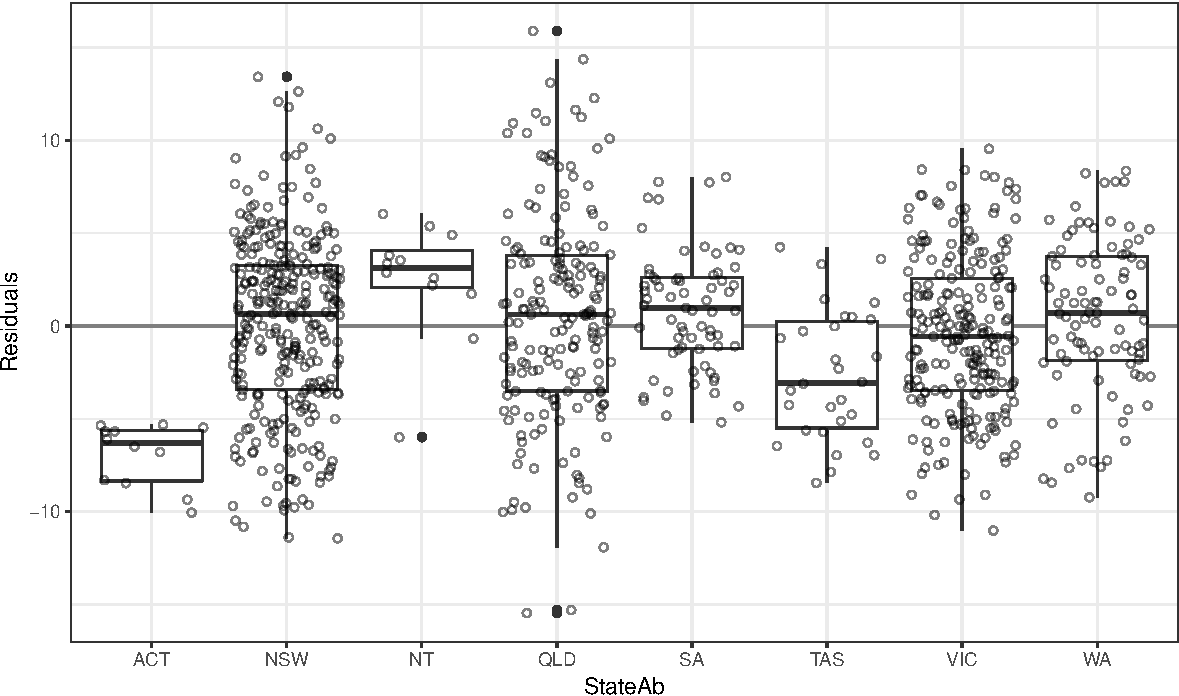
\includegraphics[width=0.7\linewidth,]{elections_conversation_files/figure-latex/resstate-1} 

}

\caption{Boxplot of residuals by state with jittered points. States ordered by median residual. A state-specific bias not captured by the model is evident.}\label{fig:resstate}
\end{figure}

\hypertarget{outlier-electorates}{%
\subsection{Outlier electorates}\label{outlier-electorates}}

Based on the distribution of the Cook's distance values, a Cook's distance greater than \(0.1\) is considered to be influential and a potential outlier. The electorate of Sydney (NSW) has a large Cook's distance from 2001 to 2013, due to its diverse population (language, birthplace and religion), high number of defacto relationships, high income, high household mobility and small amount of workers in extractive and transformative jobs. It has remained a strong supporter of the Labor party and the Liberal vote is severely overpredicted by the model, making it an outlier. Nearby in metropolitan NSW, the electorate of Wentworth is found to be an outlier in all but the 2007 election. Although historically Liberal, its two-party vote jumped by over 10 percentage points in 2010 without experiencing any notable changes in its socio-demographic makeup --- implying that this may be the direct effect of its Liberal member, Malcolm Turnbull, becoming the leader of the Liberal party. Liberal support in Wentworth is underpredicted by the model in each year, and more so with Turnbull as Liberal leader.

Lingiari, an electorate taking up almost all of the Northern Territory, is an outlier in the 2001--2007 elections due to its large Indigenous population, young age profile and low rates of property ownership. Fowler (NSW) has a diverse population with a high proportion of migrants, many Buddhists and Muslims, and has strong Labor support, making it influential in 2001, 2004 and 2010. Other electorates with large Cook's distance are Barton (NSW) and Leichhardt (QLD) in 2016, and Canberra (ACT) in 2007.

\hypertarget{conclusion}{%
\section{Conclusion}\label{conclusion}}

This paper explores the effects of electoral socio-demographic characteristics on the two-party preferred vote in the 2001--2016 elections, using information from the corresponding Australian federal elections and Censuses. As a Census does not always occur in the same year as an election, Census data for the 2004--2013 elections are generated by employing a method of spatio-temporal imputation. This imputes electoral socio-demographics for the electoral boundaries in place at the time of the election --- an approach that is distinctly different from previous work on modelling election outcomes, where Census and election data are typically joined without addressing their temporal differences. Before estimating a model, these socio-demographic variables are standardized (to adjust for changing variable scales) and many variables (representing similar information) are combined into factors, resulting in a reduced predictor set. A spatial error model is then estimated for each election, accounting for the inherent spatial structure of the data.

Across the past six elections, most of the socio-demographics that drive the electoral two-party preferred vote are found to remain steady, whilst a few (typically weaker) effects vary over time. Industry and type of work are particularly influential, with energy-related and manufacturing/construction jobs, as well as administrative roles being strongly linked with the Liberal party in all elections. Incomes have a similarly consistent effect, with higher income areas supporting Liberal. Higher levels of unemployment shift from weak association with Labor to a significant Liberal effect over the years, and higher education levels are associated with Labor from 2007 (although significant only in 2016). It is also found that electorates with higher household mobility support Liberal, birthplace diversity favours Labor and more de facto relationships align with Labor preference --- although marriages, family and household sizes have no material influence. Furthermore, the neighbourhood (spatial) effects are found to be positive in all elections, although significant only in 2001 and 2016, meaning that in the 2004--2013 elections, electorates effectively voted independently.

The findings in this paper complement the existing literature by modelling temporal trends, which as far as the authors are aware, has not been done previously for Australian elections using a regression framework. It is also the first study to model any Australian election since 2010 using Census information.

Additionally, a key contribution of this research is the wrangling of the raw data and imputed data sets for the 2004, 2007, 2010 and 2013 elections, which have been contributed to the \texttt{eechidna} \texttt{R} package --- providing a rich, accessible data resource for future Australian electoral analysis.

\hypertarget{acknowledgements}{%
\section{Acknowledgements}\label{acknowledgements}}

This paper was produced using \texttt{RMarkdown} \autocite{rmarkdown} and \texttt{knitr} \autocite{knitr}. All corresponding code for this paper can be found in the github repository \href{https://github.com/jforbes14/eechidna-paper}{github.com/jforbes14/eechidna-paper}, and the data used is available in the \texttt{eechidna} package \autocite{eechidna}. All raw data was obtained from the Australian Electoral Commission, the Australian Bureau of Statistics and the Australian Government.

\hypertarget{software}{%
\section{Software}\label{software}}

All election and Census datasets, along with electoral maps and more, are available in the \texttt{eechidna} (Exploring Election and Census Highly Informative Data Nationally for Australia) \texttt{R} package, which can be downloaded from CRAN. The \texttt{eechidna} package makes it easy to look at the data from the Australian Federal elections and Censuses that occurred between 2001 and 2016. This study contributed a large revision to the \texttt{eechidna} package, which included the addition of election and Census data for 2001--2010, voting outcomes for polling booths and imputed Census data for election years. For more details on using \texttt{eechidna}, please see the articles (vignettes) on the github page \href{https://ropenscilabs.github.io/eechidna/}{ropenscilabs.github.io/eechidna/}.

The authors would like to sincerely thank Anthony Ebert, Heike Hofmann, Thomas Lumley, Ben Marwick, Carson Sievert, Mingzhu Sun, Dilini Talagala, Nicholas Tierney, Nathaniel Tomasetti, Earo Wang and Fang Zhou, all of whom have contributed to the \texttt{eechidna} package.

\hypertarget{from-emil}{%
\section{From Emil}\label{from-emil}}

In terms of structure, start with a brief paragraph or two on what the research is, and what the reader can expect to find below.

Then, break the article into small sections for each of the factors that have an effect (a short paragraph or two for each factor). And it would be great to include examples of specific seats where the relationship was strong, or interesting for other reasons.

So the sections will be:

\begin{itemize}
\tightlist
\item
  Age
\item
  Income
\item
  Unemployment
\item
  Industry and type of work
\item
  Education
\item
  Diversity
\item
  Household mobility
\item
  Relationships
\end{itemize}

An example of this structure can be seen here:
\url{https://theconversation.com/confused-about-aged-care-in-the-home-these-10-charts-explain-how-it-works-113923}

Questions on particular factors:

Incomes:
- Was this correlation stronger in 2016? (and increasingly influential?)

Household mobility
- In the report, you say: ````Having controlled for characteristics of house ownership and rental prices'', whis effect is somewhat surprising''. Why is this surprising to you? (I would have expected this to support Labor more)

Age
- Would it be possible to show how the correlation changes for different age brackets (ie. younger voters = more Labor, and this swings more to Liberal as the age brackets gets older)?
- If not, can you go into more detail specific age brackets? Eg. Is it the over-65s that skew Liberal?

Diversity
- Migrant population: Would it possible to break this out into particular groups? eg. Seats with higher Chinese population correlates with Liberal, seats with higher SEAsia pop correlates with Labor, etc?
- The same for languages?

\printbibliography


\end{document}
